\documentclass[french]{article}
\usepackage{ae, lmodern}
\usepackage[francais]{babel}
\usepackage[utf8]{inputenc}
\usepackage[T1]{fontenc}
\usepackage{todonotes}
\usepackage{fancyhdr}
\usepackage{soul}
\usepackage{ulem}
\usepackage{color}
\usepackage{float}
\usepackage{graphicx}
\usepackage{verbatim}
\usepackage{moreverb}
\usepackage{listings}
\usepackage{url}
\usepackage{array}
\usepackage{longtable}



\title{Simulation sur ordinateur \\ Première session : Rapport \\ Etude du caractère pseudo-aléatoire de $\pi$}
\author{Maazouz Mehdi, Caredda Giuliano \\ BA3 Info}
\date{28 Mai 2018}

\begin{document}
\maketitle
\newpage
\renewcommand{\contentsname}{Sommaire}
\tableofcontents
\newpage

\section{Introduction}
Le travail que nous devons présenter consiste à étudier le caractère pseudo-aléatoire des décimales de $\pi$
en utilisant les techniques vues au cours et ce, suivant une lois uniforme. \\
De plus, nous allons devoir nous servir de ces décimales pour implémenter un générateur de loi uniforme [0,1[ 
et de comparer ce dernier au générateur par défaut de Python. \\
Nous effectuerons 3 tests pour l'étude du caractère pseudo aléatoire et 3 autres tests pour la comparaison avec le générateur par défaut de Python. Ces derniers seront décris ci-dessous. \\
Nous nous servirons du langage Python pour effectuer nos différents tests.

\subsection{Fichiers Annexes}
Afin de réaliser ce projet, nous allons devoir réaliser quelques scripts pour les différents tests qui 
vont suivre ci-dessous. Pour ce faire, nous nous sommes servis du langage de programmation Python dans sa version 2.7. 
\\
Son module Gnuplot va également servir pour les graphes qui seront tracés au fur et à mesure. D'autres modules de Python tel que le module Math ou Sympy ont été utilisés.

\section{Etude de $\pi$ }
\subsection{Approche Naïve}
Nous savons que $\pi$ contient un nombre infinis de décimales. En partant de ça, supposons que nos décimales suivent une loi uniforme. En partant de cette supposition, nous allons tracer un histogramme comprenant les occurrences de chaque digit parmi le million de décimales fournies sur la plateforme Moodle.
\\
Le nombre d'occurrence théorique de chaque digit devrait être de 100 000. En effet, on a 10 digits ( de 0 à 9), avec une probabilité de 1/10 de sortir.
\\
\\
Regardons maintenant notre premier histogramme et débattons ensuite des premières constatations.

\begin{center}
	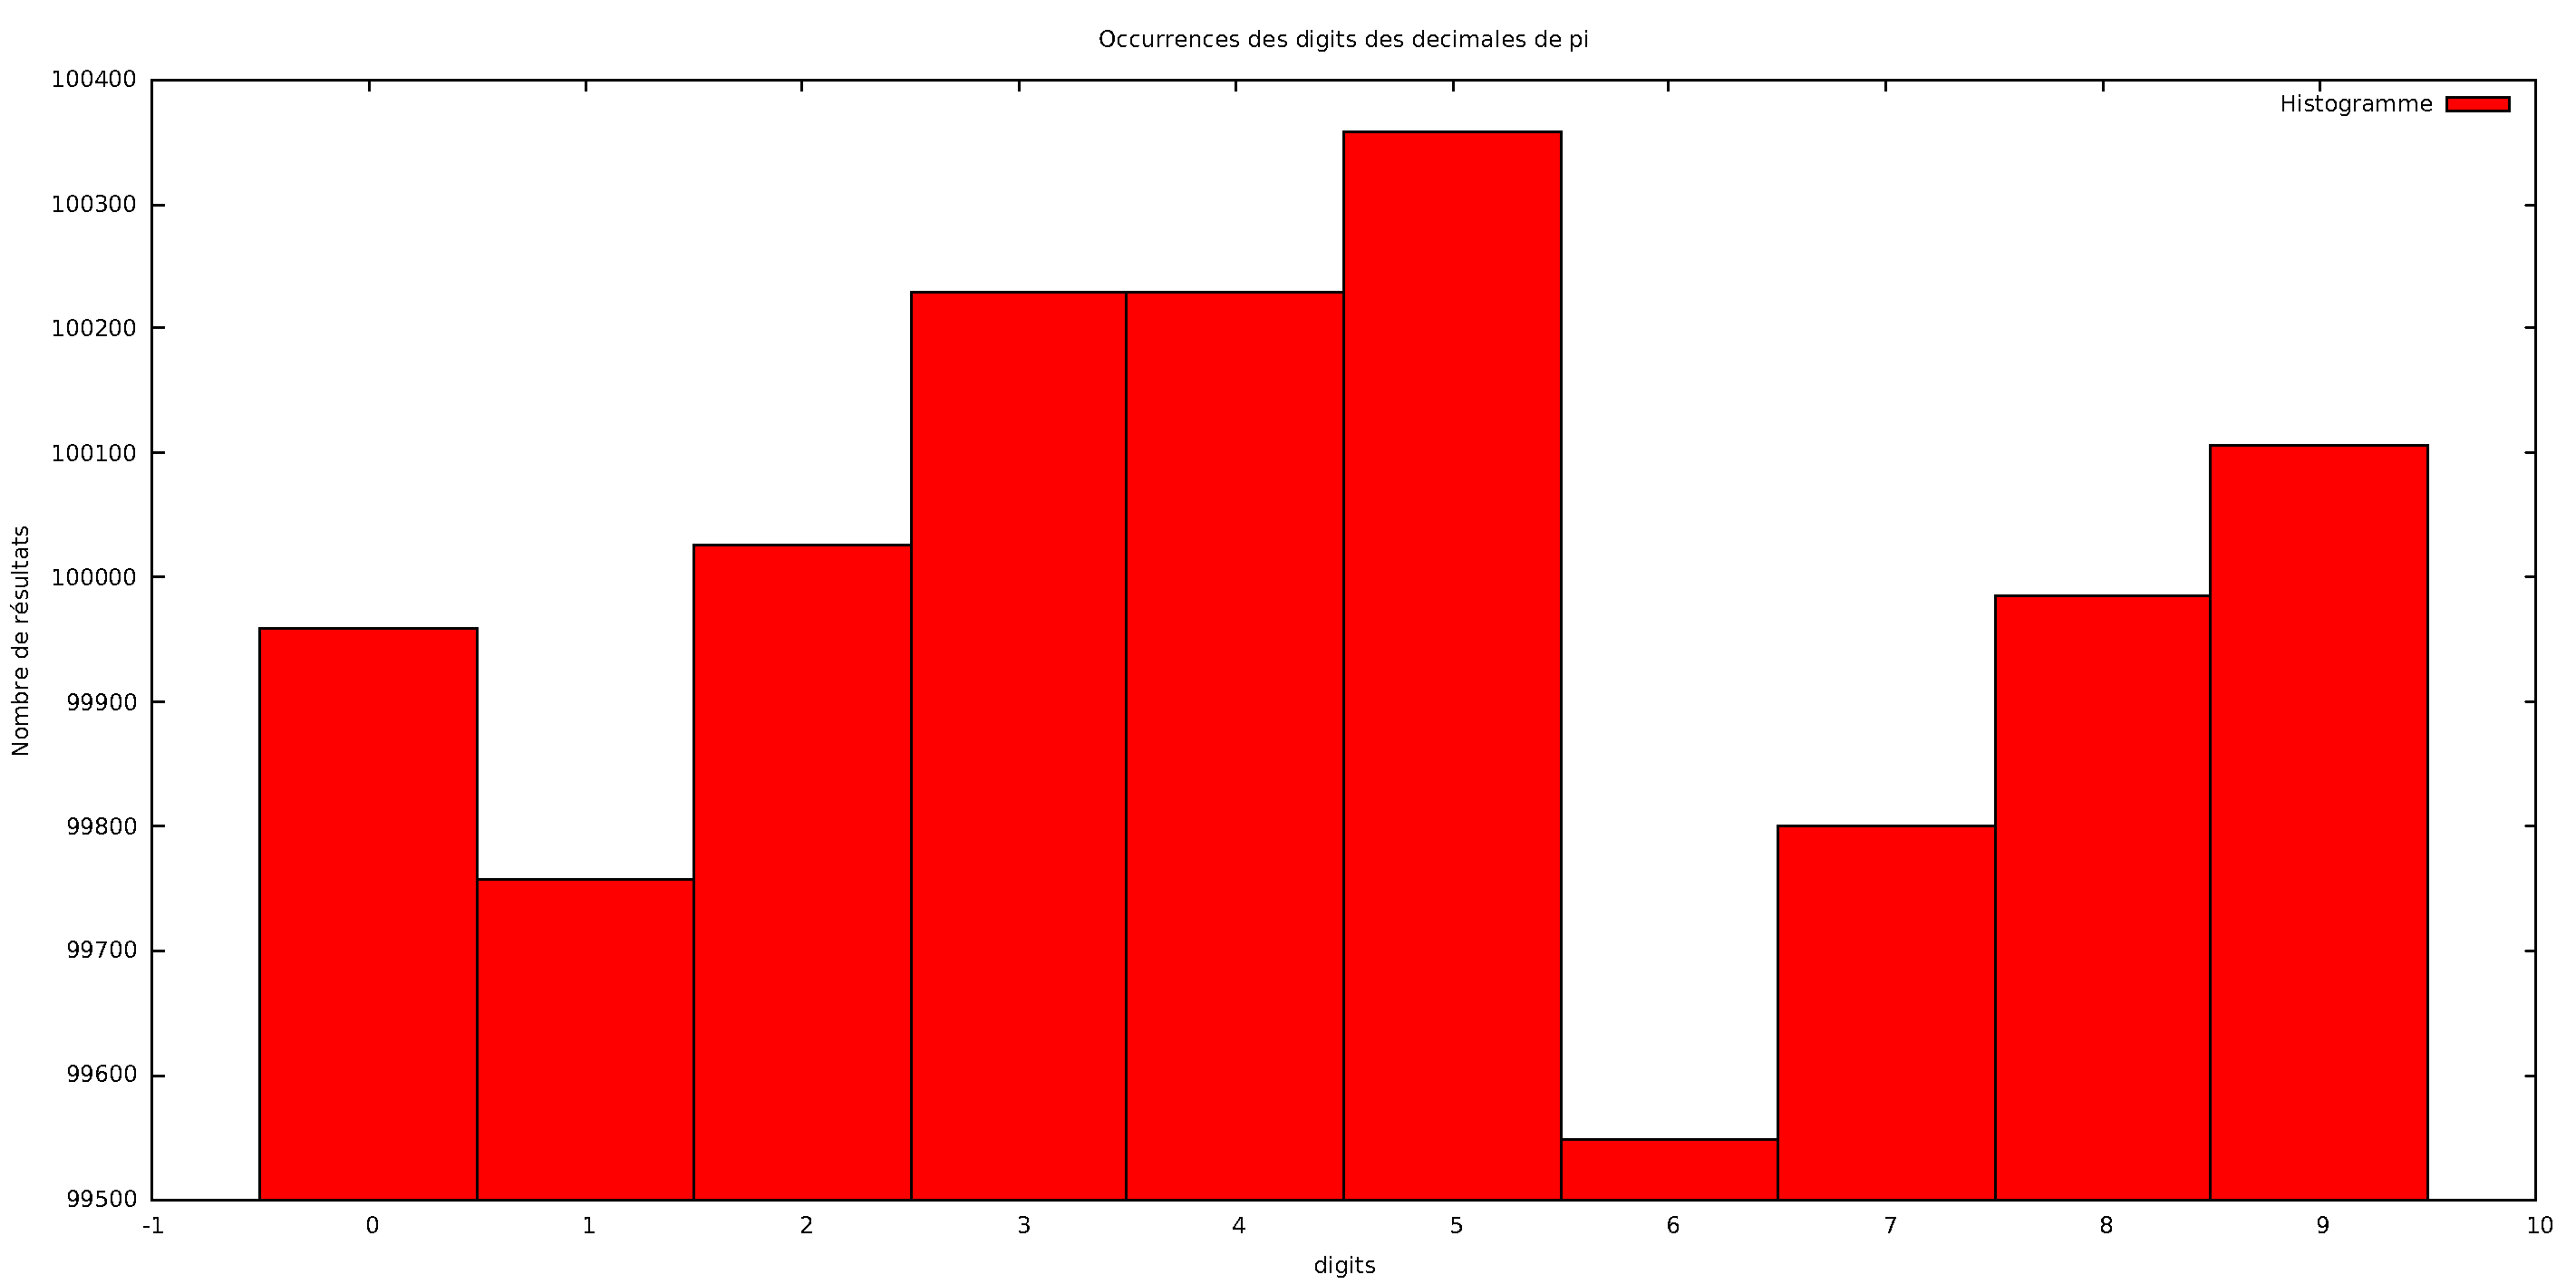
\includegraphics[scale=0.30]{Archives/Images/histo_zoom}
\end{center}

Mettons désormais les données sous la forme d'un tableau.

\begin{longtable}{|c|c|c|c|c|c|c|c|c|c|}
	\hline
	& \multicolumn{3}{c|}{\textbf{Résultats}} \\ 
	\hline 
	\textbf{Digit}  & \textbf{Observé} & \textbf{Attendu} & \textbf{Erreur en \%} \\ 
	\hline 
	$$0$$ & 99 959 & 100 000 & 0.041\\ 
	\hline 
	$$1$$ & 99 758 & 100 000 & 0.24\\ 
	\hline 
	$$2$$ & 100 026 & 100 000 & 0.026 \\ 
	\hline 
	$$3$$ & 100 229 & 100 000 & 0.229\\ 
	\hline 
	$$4$$ & 100 230 & 100 000 & 0.230\\ 
	\hline 
	$$5$$ & 100 359 & 100 000 & 0.359\\ 
	\hline 
	$$6$$ & 99 548 & 100 000 & 0.452\\ 
	\hline 
	$$7$$ & 99 800 & 100 000 & 0.2\\ 
	\hline 
	$$8$$ & 99 985 & 100 000 & 0.015\\ 
	\hline 
	$$9$$ & 100 106 & 100 000 & 0.106\\ 
	\hline
\end{longtable}

On peut constater qu'entre les résultats observés et attendus, il y a à chaque fois une
erreur inférieur à 0,5\%
\\
Ce qui nous encourage à penser que nos données suivent bien une loi uniforme même si cela ne 
constitue pas une preuve.
\\
Nous allons bientôt passer à l'étude du caractère pseudo-aléatoire des décimales de $\pi$
par l'intermédiaire de 3 tests différents.
\\
\subsection{Test de $\chi^{2}$ }
Le premier test que nous allons effectuer est le test du \textbf{$\chi^{2}$}. Ce dernier est un test statistique qui va permettre de vérifier si une série de données est susceptible de suivre une loi de probabilité.
\\
Pour effectuer ce test, nous allons devoir regrouper ces données dans différentes classes.
Voici un rappel théorique :

	\begin{center}
		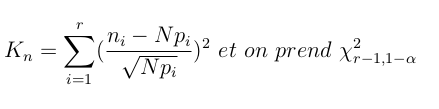
\includegraphics[scale=0.60]{Archives/Images/khi2}
	\end{center}
	
On peut y apercevoir \textit{r} qui correspond au nombre de classes. \\
\textit{N$p_{i}$} qui correspond aux nombres d'occurrences théoriques. \\
\textit{$n_{i}$} qui correspond aux nombres d'occurrences observées.
\\
\\
Partons désormais de notre hypothèse nulle nommée $H_{0}$ = {nos décimales de $\pi$ suivent une loi uniforme}.
\\
Dans notre cas, \textit{r} sera fixé à 10, car nous considérerons une classe par digit, et \textit{N$p_{i}$} sera fixé à 100 000.\\ 
Quant à \textit{$n_{i}$}, ses différentes valeurs seront issues du nombre d'occurrence observés dans l'histogramme présenté précédemment.
Comme le demande le test de \textbf{$\chi^{2}$}, nous devons fixer une probabilité $\alpha$, appeler erreur de première espèce, de rejeter l'hypothèse nulle $H_{0}$.
\\
Une fois ce paramètre $\alpha$ fixé, nous pouvons désormais vérifier si $H_{0}$ est acceptée
si $K_{n}$ <= $\chi^{2}_{9,\alpha-1}$ où 9 est le degré de liberté calculé en faisant \textit{r}-1 (nombre de classes -1).

Voici les différents résultats obtenus en fonction de différentes valeurs pour $\alpha$.
\\
\begin{longtable}{|c|c|c|c|c|c|c|c|c|c|}
	\hline
	& \multicolumn{3}{c|}{\textbf{Résultats}} \\ 
	\hline 
	\textbf{$\alpha$}  & $K_{n}$ & $\chi^{2}_{9,\alpha-1}$ & \textbf{Resultat} \\ 
	\hline 
	$$0.001$$ & 5.50908 & 27.877 & Reussite\\ 
	\hline 
	$$0.025$$ & 5.50908 & 19.023 & Reussite\\ 
	\hline 
	$$0.1$$ & 5.50908 & 14.684 & Reussite \\ 
	\hline 
\end{longtable}

On peut constater que les tests réussis, nous sommes donc confortés dans notre supposition qui était que les décimales de $\pi$ suivent une loi uniforme.
\\

\subsection{Test du Poker}
Une fois le test du $\chi^{2}$ effectué, passons maintenant à un autre test qui va s'appuyer sur ce dernier, le test du Poker. Pour ce faire, nous allons diviser notre million de décimales en 200 000 blocs contenant chacun 5 décimales. Nous dirons que chaque bloc contient une séquence.
\\
\\
Une fois les blocs obtenus, nous allons les classer en fonction du \textit{nombre} de digit différents par bloc. Ce \textit{nombre} est appelé \textit{r} et est compris entre 1 et 5.
\\
En effet, une séquence peut seulement contenir un digit différent ( par exemple : 11111) mais également 5 digits différents (12345).
\\
Nous allons désormais passer au calcul du $\chi^{2}$ en se basant sur le nombre de \textit{Stirling} pour
effectuer la comparaison. Ce dernier se définit comme étant le \textit{nombre de manières possibles de constituer r paquets avec k nombres}.
\\
Par le rappel théorique (\textit{voir cours}), nous obtenons $P_{r}$, la probabilité d'avoir \textit{r}.

	\begin{center}
		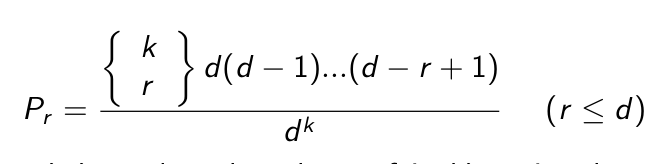
\includegraphics[scale=0.60]{Archives/Images/probaR}
	\end{center}

Avec \textbf{K} la longueur de la séquence , \textbf{d} le nombre de digits possibles et enfin \textbf{r}
définis plus haut.
\\
Pour effectuer nos calculs, nous fixerons \textbf{K} à 5 et \textbf{d} à 10.
\\
Une fois les probabilités obtenues, multiplions ces dernières par le nombre de paquet (200 000).

\centering
	\begin{tabular}{|r|r|r|}
		\hline
		r & valeur théorique & valeur calculée\\
		\hline
		1 & 20 & 13\\
		2 & 2700 & 2644\\
		3 & 36000 & 36172\\
		4 & 100800 & 100670\\
		5 & 60480 & 60501\\
		\hline
	\end{tabular}


	\begin{center}
		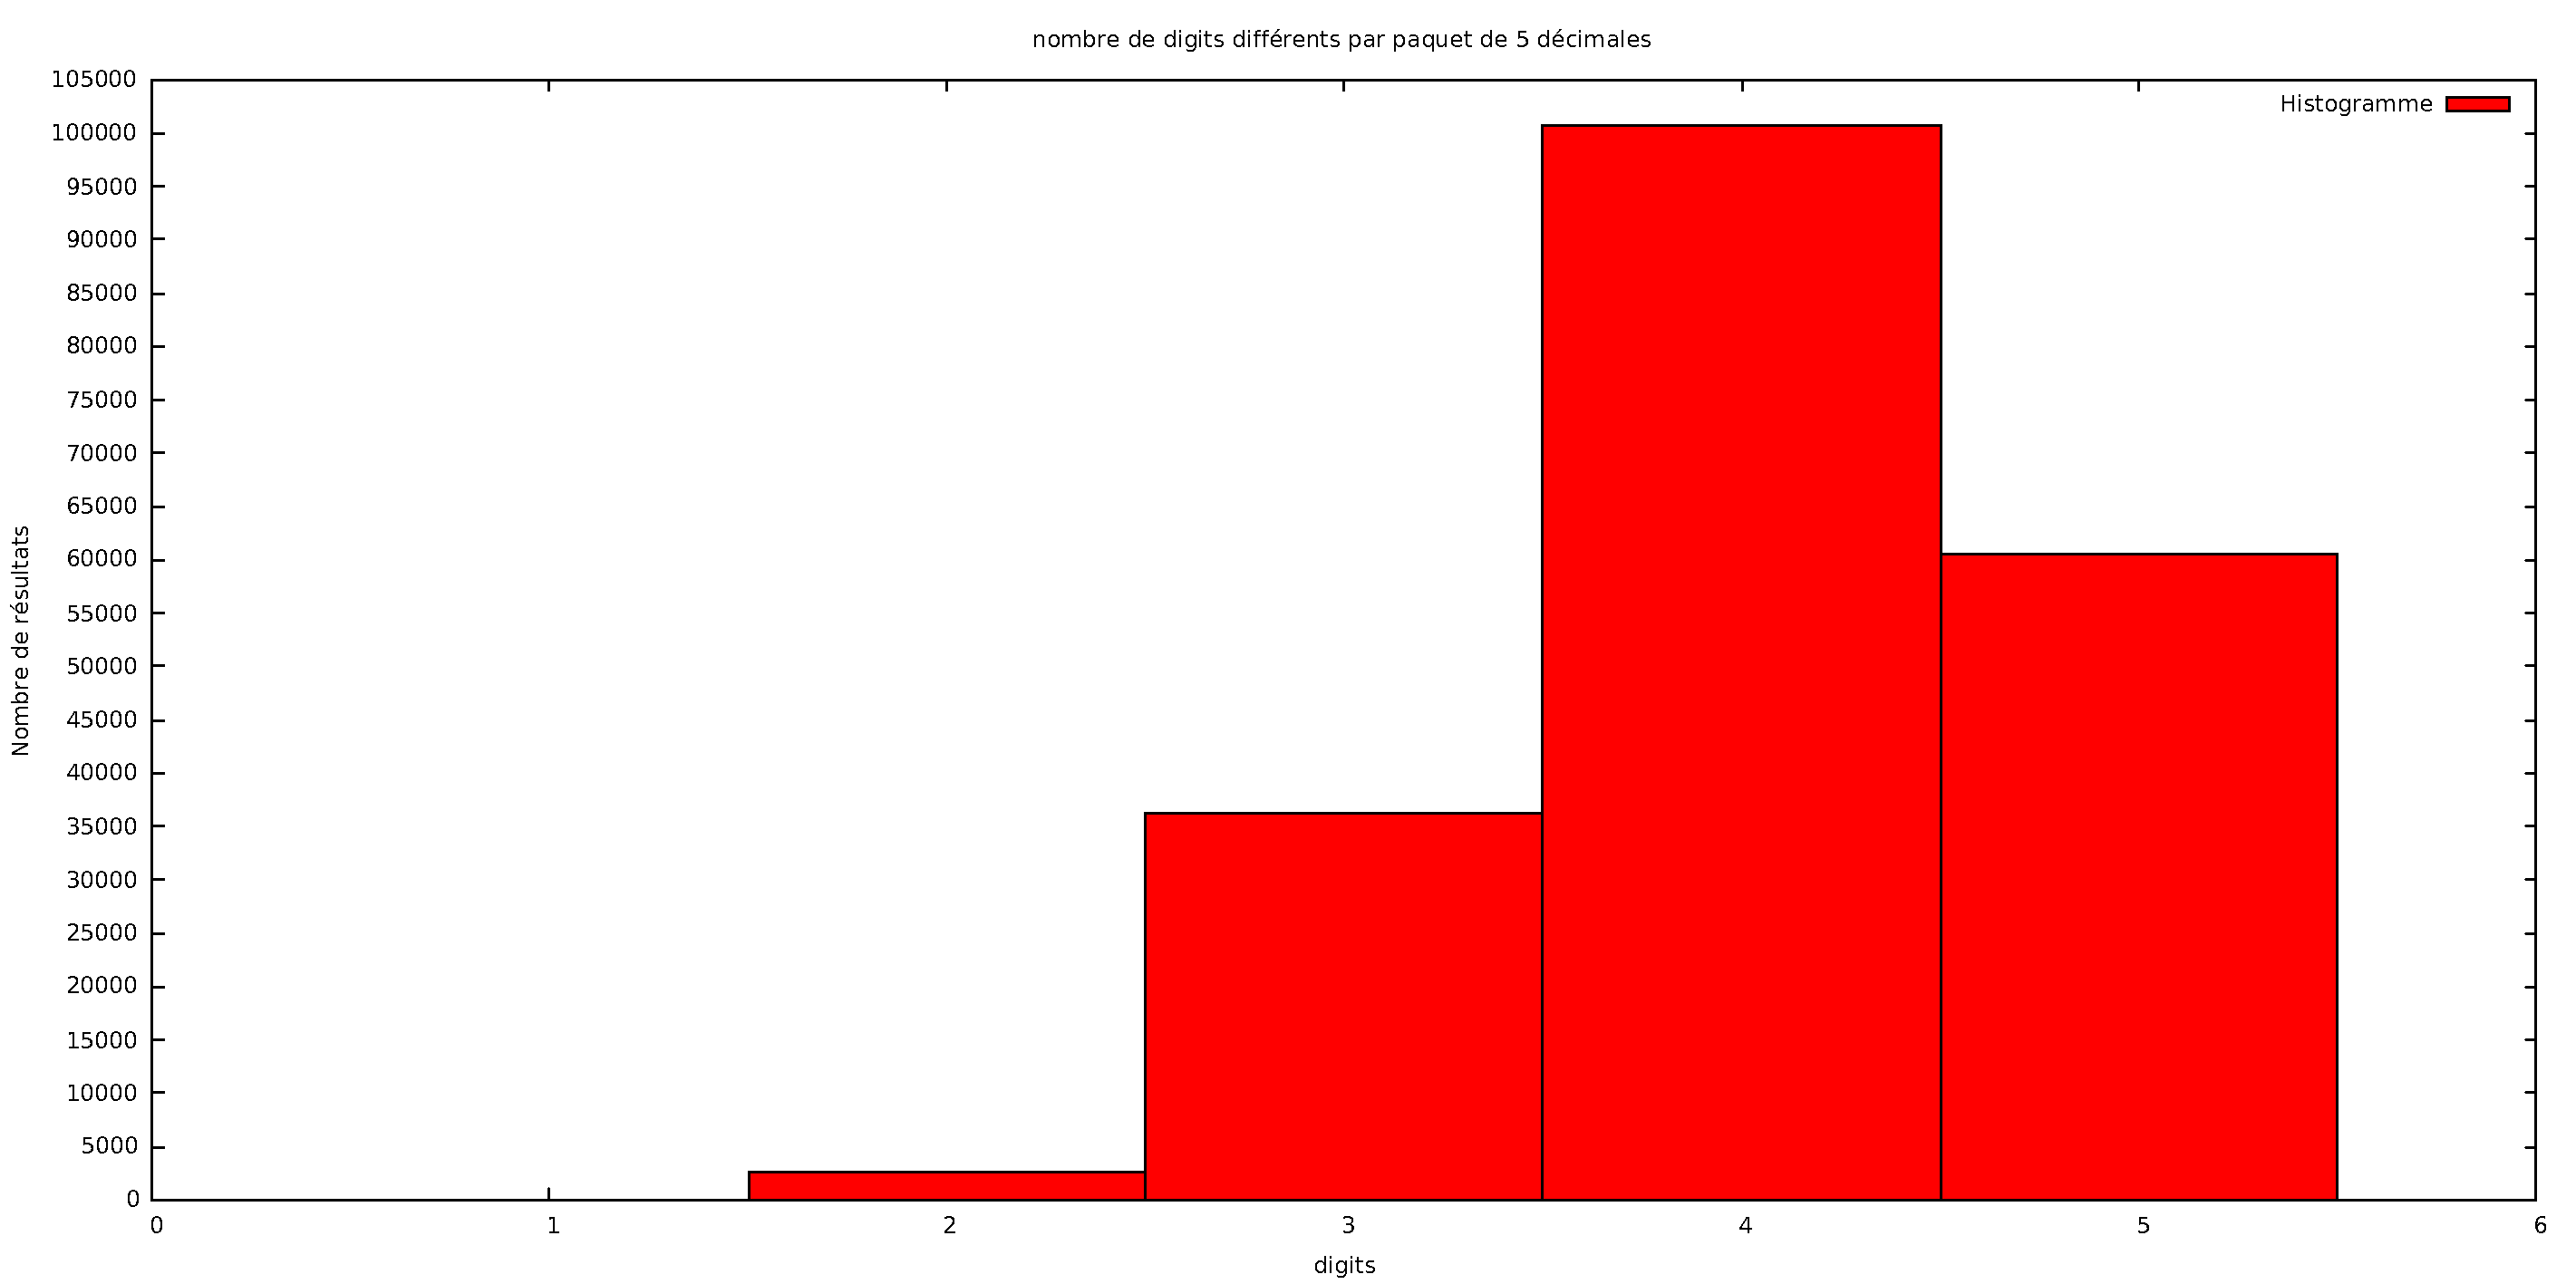
\includegraphics[scale=0.30]{Archives/Images/histo_poker}
	\end{center}


\subsection{Test du collectionneur de coupons}
Le dernier test que nous allons employer repose sur le principe suivant. 
\\
Tout d'abord, nous allons parcourir les décimales de $\pi$ avec pour objectif de construire des séquences.
Une séquence étant construite dès que l'on a parcouru une fois tous les digits possible (de 0 à 9 compris).
Il suffit ensuite de recommencer la procédure avec les décimales suivantes.
\\
On peut facilement comprendre que nous obtiendrons des séquences avec des tailles différentes.
\\

Afin de vérifier si nos séquences suivent bien une loi uniforme, nous devons tout d'abord calculé la probabilité $S_{r}$, autrement dit, la probabilité d'avoir une séquence de taille \textit{r} ayant tous nos digits est donnée par la formule suivante :

	\begin{center}
		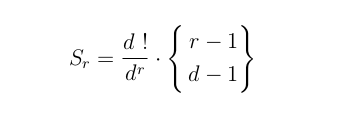
\includegraphics[scale=0.40]{Archives/Images/coupons}
	\end{center}

d représente le nombre de digits possibles, ici, il sera égal à 10.
Afin d'obtenir la valeur théorique pour chaque taille de séquence \textit{$ r_{i} $}, il suffit de multiplier la probabilité $S_{r_{i}}$  par le nombre total de séquences obtenues.
\\

La dernière étape de notre test consistera à comparer cette valeur théorique à notre valeur obtenue à l'aide du test du $\chi^{2}$.

Nos longueurs de séquences formeront nos classes pour le test de $\chi^{2}$. Nous avons 100 classes, cependant, les séquences ayant une taille allant de 1 à 9 ont une valeur théorique et observée de 0. Elles sont donc inutiles à prendre en considération pour le test de $\chi^{2}$.  Le degré de liberté sera donc égal à 91-1 ($\chi^{2}_{91,\alpha-1}$).
\newpage
\begin{figure}[h]
	\centering
	\begin{tabular}{|r|r|r|}
		\hline
		Tailles de séquences & Valeur théorique & Valeur observée\\
		\hline
		10 & 12.39706944 & 12\\
		11 & 55.78681248 & 62\\
		12 & 143.186152032 & 154\\
		13 & 276.144721776 & 265\\
		14 & 445.677125782 & 496\\
		15 & 636.605631934 & 645\\
		16 & 832.196551932 & 869\\
		17 & 1017.53193425 & 1008\\
		18 & 1181.29471772 & 1150\\
		19 & 1316.26375399 & 1341\\
		20 & 1418.98670105 & 1354\\
		21 & 1489.0470501 & 1482\\
		22 & 1528.21745078 & 1576\\
		23 & 1539.67053158 & 1515\\
		24 & 1527.32748565 & 1543\\
		25 & 1495.36642995 & 1456\\
		26 & 1447.88033297 & 1470\\
		27 & 1388.65981367 & 1345\\
		28 & 1321.07229861 & 1317\\
		29 & 1248.01086229 & 1224\\
		30 & 1171.89036844 & 1145\\
		31 & 1094.67343335 & 1105\\
		32 & 1017.91330149 & 1018\\
		33 & 942.804564011 & 968\\
		34 & 870.235668768 & 883\\
		35 & 800.839427633 & 817\\
		36 & 735.039345563 & 772\\
		37 & 673.090709825 & 680\\
		38 & 615.116112395 & 640\\
		39 & 561.135537135 & 522\\
		40 & 511.091408294 & 506\\
		41 & 464.869130432 & 456\\
		42 & 422.313697469 & 406\\
		43 & 383.242942754 & 379\\
		44 & 347.457965104 & 351\\
		45 & 314.751212876 & 324\\
		46 & 284.912648965 & 280\\
		47 & 257.734360295 & 266\\
		48 & 233.013919451 & 219\\
		49 & 210.556755384 & 212\\
		50 & 190.177745431 & 185\\
		\hline
	\end{tabular}
	\caption{Tableau de Test du CDC : Les décimales de Pi 1}
\end{figure}

\newpage
\begin{figure}[h]
	\centering
	\begin{tabular}{|r|r|r|}
		\hline
		Tailles de séquences & Valeur théorique & Valeur observée\\
		\hline
		51 & 171.702202299 & 197\\
		52 & 154.966396843 & 142\\
		53 & 139.817729962 & 148\\
		54 & 126.114644036 & 115\\
		55 & 113.726345551 & 113\\
		56 & 102.532395165 & 87\\
		57 & 92.4222090177 & 95\\
		58 & 83.294505053 & 77\\
		59 & 75.0567200775 & 80\\
		60 & 67.624416886 & 69\\
		61 & 60.9206957291 & 66\\
		62 & 54.8756204189 & 62\\
		63 & 49.4256662748 & 59\\
		64 & 44.5131947077 & 44\\
		65 & 40.0859574053 & 39\\
		66 & 36.0966316837 & 34\\
		67 & 32.5023875297 & 32\\
		68 & 29.2644860878 & 22\\
		69 & 26.3479087976 & 22\\
		70 & 23.7210160015 & 27\\
		71 & 21.3552335886 & 25\\
		72 & 19.2247660837 & 27\\
		73 & 17.3063345114 & 17\\
		74 & 15.5789373362 & 8\\
		75 & 14.0236327962 & 12\\
		76 & 12.6233409926 & 12\\
		77 & 11.3626641589 & 5\\
		78 & 10.2277236148 & 13\\
		79 & 9.20601199223 & 9\\
		80 & 8.28625941323 & 12\\
		81 & 7.45831238842 & 8\\
		82 & 6.71302429704 & 7\\
		83 & 6.04215639528 & 8\\
		84 & 5.43828838508 & 4\\
		\hline
	\end{tabular}
	\caption{Tableau de Test du CDC : Les décimales de Pi 3}
\end{figure}

\begin{figure}[h]
	\centering
	\begin{tabular}{|r|r|r|}
		\hline
		Tailles de séquences & Valeur théorique & Valeur observée\\
		\hline
		85 & 4.89473765491932 & 4\\
		86 & 4.40548637952699 & 5\\
		87 & 3.96511573604793 & 6\\
		88 & 3.56874655969782 & 3\\
		89 & 3.21198582270483 & 1\\
		90 & 2.89087837643692 & 0\\
		91 & 2.60186344817007 & 1\\
		92 & 2.34173543125690 & 4\\
		93 & 2.10760855073593 & 4\\
		94 & 1.89688502594326 & 0\\
		95 & 1.70722638771169 & 1\\
		96 & 1.53652764052733 & 1\\
		97 & 1.38289398981167 & 4\\
		98 & 1.244619881547491 & 0\\
		99 & 1.12017012599947 & 2\\
		\hline
	\end{tabular}
	\caption{Tableau de Test du CDC : Les décimales de Pi 3}
\end{figure}

\newpage
Nous pouvons constater que le tableau affiche les résultats à partir des séquences de longueur 10. En effet, il est inutile de prendre en considération les séquences de longueur inférieure à 10 car il est impossible de trouver une séquence contenant les 10 digits différents (0 à 9) si la séquence a une longueur inférieure à 10.

\\
\begin{longtable}{|c|c|c|c|c|c|c|c|c|c|}
	\hline
	& \multicolumn{3}{c|}{\textbf{Résultats}} \\ 
	\hline 
	\textbf{$\alpha$}  & $K_{n}$ & $\chi^{2}_{9,\alpha-1}$ & \textbf{Resultat} \\ 
	\hline 
	$$0.001$$ & 78.792 & 137.21 & Reussite\\ 
	\hline 
	$$0.025$$ & 78.792 & 118.14 & Reussite\\ 
	\hline 
	$$0.1$$ & 78.792 & 107.57 & Reussite \\ 
	\hline 
\end{longtable}

\section{Générateur de nombre pseudo-aléatoire}
\subsection{Enonce}
La deuxième partie de notre projet consiste à implémenter un générateur de nombre pseudo-aléatoire et ensuite, de le comparer avec le générateur par défaut de Python (Mersenne Twister). Plus concrètement, nous devons implémenter un générateur qui devra, comme son nom l'indique, générer des nombres compris entre 0 et 1
de manière uniforme.

\subsection{Implémentation}
Nous savons que l'ordinateur est une machine déterministe. Cependant, nous pouvons faire ressortir une composante aléatoire en utilisant le temps écoulé, en millisecondes, depuis le $1^{er}$ Janvier 1970.
\\
Etant donné que les premières décimales de  $\pi$ nous sont fournies, nous allons pouvoir nous en servir pour l'implémentation de notre générateur.
\end{document}
